\documentclass[a4paper, 12pt, twoside]{article}


%------------------------------------------------------------------------
%
% Author                :   Lasercata
% Last modification     :   2024.05.21
%
%------------------------------------------------------------------------

%---------Init {{{1
%------Lang
\usepackage[french]{babel}
%\usepackage[english]{babel}


%See https://github.com/lasercata/LaTeX_Templates for the file latex_base.sty
%------------------------------------------------------------------------
% This is a LaTeX template, with some useful commands and environments.
%
% Author                :   Lasercata
% Last modification     :   2023.12.18
% Version               :   v6.0.4
%
%------------------------------------------------------------------------


%------ini
\usepackage[utf8]{inputenc}
\usepackage[T1]{fontenc}


%------geometry
\usepackage[textheight=700pt, textwidth=500pt]{geometry}


%------color
\usepackage{xcolor}
\definecolor{ff4500}{HTML}{ff4500}
\definecolor{00f}{HTML}{0000ff}
\definecolor{0ff}{HTML}{00ffff}
\definecolor{656565}{HTML}{656565}

\newcommand{\Emph}{\textcolor{ff4500}}

\newcommand{\strong}[1]{\textcolor{ff4500}{\bf #1}}
\newcommand{\st}{\color{ff4500}\bf}


%------Code highlighting
%---listings
\usepackage{listings}

\definecolor{cbg}{HTML}{272822}
\definecolor{cfg}{HTML}{ececec}
\definecolor{ccomment}{HTML}{686c58}
\definecolor{ckw}{HTML}{f92672}
\definecolor{cstring}{HTML}{e6db72}
\definecolor{cstringlight}{HTML}{98980f}
\definecolor{lightwhite}{HTML}{fafafa}

\lstdefinestyle{DarkCodeStyle}{
    backgroundcolor=\color{cbg},
    commentstyle=\itshape\color{ccomment},
    keywordstyle=\color{ckw},
    numberstyle=\tiny\color{cbg},
    stringstyle=\color{cstring},
    basicstyle=\ttfamily\footnotesize\color{cfg},
    breakatwhitespace=false,
    breaklines=true,
    captionpos=b,
    keepspaces=true,
    numbers=left,
    numbersep=5pt,
    showspaces=false,
    showstringspaces=false,
    showtabs=false,
    tabsize=4,
    xleftmargin=\leftskip
}

\lstdefinestyle{LightCodeStyle}{
    backgroundcolor=\color{lightwhite},
    commentstyle=\itshape\color{ccomment},
    keywordstyle=\color{ckw},
    numberstyle=\tiny\color{cbg},
    stringstyle=\color{cstringlight},
    basicstyle=\ttfamily\footnotesize\color{cbg},
    breakatwhitespace=false,
    breaklines=true,
    captionpos=b,
    keepspaces=true,
    numbers=left,
    numbersep=10pt,
    showspaces=false,
    showstringspaces=false,
    showtabs=false,
    tabsize=4,
    frame=L,
    xleftmargin=\leftskip
}

%\lstset{style=DarkCodeStyle}
\lstset{style=LightCodeStyle}
%Usage : \begin{lstlisting}[language=Caml, xleftmargin=xpt] ... \end{lstlisting}


%---Algorithm
\usepackage[linesnumbered,ruled,vlined]{algorithm2e}
\SetKwInput{KwInput}{Input}
\SetKwInput{KwOutput}{Output}

\SetKwProg{Fn}{Function}{:}{}
\SetKwProg{Proc}{Procedure}{:}{}
\SetKw{KwPrint}{Print}

\newcommand\commfont[1]{\textit{\texttt{\textcolor{656565}{#1}}}}
\SetCommentSty{commfont}
\SetProgSty{texttt}
\SetArgSty{textnormal}
\SetFuncArgSty{textnormal}
%\SetProgArgSty{texttt}

\newenvironment{indalgo}[2][H]{
    \begin{algoBox}
        \begin{algorithm}[#1]
            \caption{#2}
}
{
        \end{algorithm}
    \end{algoBox}
}


%---tcolorbox
\usepackage[many]{tcolorbox}

\DeclareTColorBox{emphBox}{O{black}O{lightwhite}}{
    breakable,
    outer arc=0pt,
    arc=0pt,
    top=0pt,
    toprule=-.5pt,
    right=0pt,
    rightrule=-.5pt,
    bottom=0pt,
    bottomrule=-.5pt,
    colframe=#1,
    colback=#2,
    enlarge left by=10pt,
    width=\linewidth-\leftskip-10pt,
}

\DeclareTColorBox{algoBox}{O{black}O{lightwhite}}{
    breakable,
    arc=0pt,
    top=0pt,
    toprule=-.5pt,
    right=0pt,
    rightrule=-.5pt,
    bottom=0pt,
    bottomrule=-.5pt,
    left=0pt,
    leftrule=-.5pt,
    colframe=#1,
    colback=#2,
    width=\linewidth-\leftskip-10pt,
}


%-------make the table of content clickable
\usepackage{hyperref}
\hypersetup{
    colorlinks,
    citecolor=black,
    filecolor=black,
    linkcolor=black,
    urlcolor=black
}


%------pictures
\usepackage{graphicx}
%\usepackage{wrapfig}

\usepackage{tikz}

\usepackage{float} % For [H] in figure env


%------tabular
%\usepackage{color}
%\usepackage{colortbl}
%\usepackage{multirow}


%------Physics
%---Packages
%\usepackage[version=4]{mhchem} %$\ce{NO4^2-}$

%---Commands
\newcommand{\link}[2]{\mathrm{#1} \! - \! \mathrm{#2}}
\newcommand{\pt}[1]{\cdot 10^{#1}} % Power of ten
\newcommand{\dt}[2][t]{\dfrac{\mathrm d #2}{\mathrm d #1}} % Derivative
\renewcommand{\d}{\mathrm d}

\newcommand{\rot}{\vect{\mathrm{rot}}}
\newcommand{\grad}{\vect{\mathrm{grad}}}
\renewcommand{\div}{\mathrm{div}}
\renewcommand{\j}{\vec\jmath}


%------math
%---Packages
%\usepackage{textcomp}
%\usepackage{amsmath}
\usepackage{amssymb}
\usepackage{mathtools} % For abs
\usepackage{stmaryrd} %for \llbracket and \rrbracket
\usepackage{mathrsfs} %for \mathscr{x} (different from \mathcal{x})
\usepackage{esint} % Better integrals (double, triple, \oiint, ...)

%---Commands
%-Sets
\newcommand{\N}{\mathbb{N}} %set N
\newcommand{\Z}{\mathbb{Z}} %set Z
\newcommand{\Q}{\mathbb{Q}} %set Q
\newcommand{\R}{\mathbb{R}} %set R
\newcommand{\C}{\mathbb{C}} %set C
\newcommand{\U}{\mathbb{U}} %set U
\newcommand{\seg}[2]{\left[ #1\ ;\ #2 \right]}
\newcommand{\nset}[2]{\left\llbracket #1\ ;\ #2 \right\rrbracket}

%-Exponantial / complexs
\newcommand{\e}{\mathrm{e}}
\newcommand{\cj}[1]{\overline{#1}} %overline for the conjugate.

%-Vectors
\newcommand{\vect}{\overrightarrow}
\newcommand{\veco}[3]{\displaystyle \vect{#1}\binom{#2}{#3}} %vector + coord

%-Limits
\newcommand{\lm}[2][{}]{\lim\limits_{\substack{#2 \\ #1}}} %$\lm{x \to a} f$ or $\lm[x < a]{x \to a} f$
\newcommand{\Lm}[3][{}]{\lm[#1]{#2} \left( #3 \right)} %$\Lm{x \to a}{f}$ or $\Lm[x < a]{x \to a}{f}$
\newcommand{\tendsto}[1]{\xrightarrow[#1]{}}

%-Integral
\newcommand{\dint}[4][x]{\displaystyle \int_{#2}^{#3} #4 \mathrm{d} #1} %$\dint{a}{b}{f(x)}$ or $\dint[t]{a}{b}{f(t)}$

%-left right
\newcommand{\lr}[1]{\left( #1 \right)}
\newcommand{\lrb}[1]{\left[ #1 \right]}
\newcommand{\lrbb}[1]{\left\llbracket #1 \right\rrbracket}
\newcommand{\set}[1]{\left\{ #1 \right\}}
\newcommand{\abs}[1]{\left\lvert #1 \right\rvert}
\newcommand{\norm}[1]{\left\lVert #1 \right\rVert}
\newcommand{\ceil}[1]{\left\lceil #1 \right\rceil}
\newcommand{\floor}[1]{\left\lfloor #1 \right\rfloor}
\newcommand{\lrangle}[1]{\left\langle #1 \right\rangle}

%-Boxes
\newcommand{\oboxed}[1]{\textcolor{ff4500}{\boxed{\textcolor{black}{#1}}}} %orange boxed

\newcommand{\rboxed}[1]{\begin{array}{|c} \hline #1 \\ \hline \end{array}} %boxed with right opened
\newcommand{\lboxed}[1]{\begin{array}{c|} \hline #1 \\ \hline \end{array}} %boxed with left opened

\newcommand{\orboxed}[1]{\textcolor{ff4500}{\rboxed{\textcolor{black}{#1}}}} %orange right boxed
\newcommand{\olboxed}[1]{\textcolor{ff4500}{\lboxed{\textcolor{black}{#1}}}} %orange left boxed

%-Others
\newcommand{\para}{/\!/} %//
\newcommand{\ssi}{\ \Leftrightarrow \ }
\newcommand{\eqsys}[2]{\begin{cases} #1 \\ #2 \end{cases}}

\newcommand{\med}[2]{\mathrm{med} \left[ #1\ ;\ #2 \right]}  %$\med{A}{B} -> med[A ; B]$
\newcommand{\Circ}[2]{\mathscr{C}_{#1, #2}}

\renewcommand{\le}{\leqslant}
\renewcommand{\ge}{\geqslant}


%------commands
%---to quote
\newcommand{\simplecit}[1]{\guillemotleft$\;$#1$\;$\guillemotright}
\newcommand{\cit}[1]{\simplecit{\textcolor{656565}{#1}}}
\newcommand{\quo}[1]{\cit{\it #1}}

%---to indent
\newcommand{\ind}[1][20pt]{\advance\leftskip + #1}
\newcommand{\deind}[1][20pt]{\advance\leftskip - #1}

%---to indent a text
\newcommand{\indented}[2][20pt]{\par \ind[#1] #2 \par \deind[#1]}
\newenvironment{indt}[2][20pt]{#2 \par \ind[#1]}{\par \deind} %Titled indented env

%---title
\newcommand{\thetitle}[2]{\begin{center}\textbf{{\LARGE \underline{\Emph{#1} :}} {\Large #2}}\end{center}}

%---Maths environments
%-Proofs
\newenvironment{proof}[1][{}]{\begin{indt}{$\square$ #1}}{$\blacksquare$ \end{indt}}

%-Maths parts (proposition, definition, ...)
\newenvironment{mathpart}[1]{\begin{indt}{\boxed{\text{\textbf{#1}}}}}{\end{indt}}
\newenvironment{mathbox}[1]{\boxed{\text{\textbf{#1}}}\begin{emphBox}}{\end{emphBox}}
\newenvironment{mathul}[1]{\begin{indt}{\underline{\textbf{#1}}}}{\end{indt}}

\newenvironment{theo}{\begin{mathpart}{Théorème}}{\end{mathpart}}
\newenvironment{Theo}{\begin{mathbox}{Théorème}}{\end{mathbox}}

\newenvironment{prop}{\begin{mathpart}{Proposition}}{\end{mathpart}}
\newenvironment{Prop}{\begin{mathbox}{Proposition}}{\end{mathbox}}
\newenvironment{props}{\begin{mathpart}{Propriétés}}{\end{mathpart}}

\newenvironment{defi}{\begin{mathpart}{Définition}}{\end{mathpart}}
\newenvironment{meth}{\begin{mathpart}{Méthode}}{\end{mathpart}}

\newenvironment{Rq}{\begin{mathul}{Remarque :}}{\end{mathul}}
\newenvironment{Rqs}{\begin{mathul}{Remarques :}}{\end{mathul}}

\newenvironment{Ex}{\begin{mathul}{Exemple :}}{\end{mathul}}
\newenvironment{Exs}{\begin{mathul}{Exemples :}}{\end{mathul}}


%------page style
\usepackage{fancyhdr}
\usepackage{lastpage}

\setlength{\headheight}{18pt}
\setlength{\footskip}{50pt}

\pagestyle{fancy}
\fancyhf{}
\fancyhead[LE, RO]{\textit{\textcolor{black}{\today}}}
\fancyhead[RE, LO]{\large{\textsl{\Emph{\texttt{\jobname}}}}}

\fancyfoot[RO, LE]{\textit{\texttt{\textcolor{black}{Page \thepage /}\pageref{LastPage}}}}
% \fancyfoot[LO, RE]{\includegraphics[scale=0.12]{/home/lasercata/Pictures/1.images_profil/logo/mieux/lasercata_logo_fly_fond_blanc.png}}
\newcommand{\setlogo}{\fancyfoot[LO, RE]{\includegraphics[scale=0.12]{/home/lasercata/Pictures/1.images_profil/logo/mieux/lasercata_logo_fly_fond_blanc.png}}}


%------init lengths
\setlength{\parindent}{0pt} %To avoid using \noindent everywhere.
\setlength{\parskip}{3pt}



%------Circuitikz
%\usetikzlibrary{babel}             %Uncomment this to use circuitikz
%\usetikzlibrary{shapes.geometric}  % To draw triangles in trees
%\usepackage[european]{circuitikz}            %Electrical circuits drawing

%------Sections
%---To change section numbering :
% \renewcommand\thesection{\Roman{section}}
% \renewcommand\thesubsection{\arabic{subsection})}
% \renewcommand\thesubsubsection{\textit \alph{subsubsection})}

%---To start numbering sections from 0
% \setcounter{section}{-1}

%---To hide subsubsection from the table of contents (show with max depth of 2)
% \setcounter{tocdepth}{2}


%------File structure
\usepackage{forest} %For the file structure


%------Logo
% \setlogo %Comment to remove the logo
%}}}1

%------Title (with default LaTeX style)
%\title{}
%\author{}
%\date{\today}

%---------------------------------Begin Document
\begin{document}
    
    % Title {{{1
    \thetitle{Structures de données}{comparaisons de structures}
    %\maketitle
    
    \tableofcontents
    \listoffigures
    \listoftables
    %\listofalgorithms
    \newpage
    % }}}1
    
    \begin{indt}{\section{Méthode de développement}}% {{{1
        \begin{indt}{\subsection{Structure du projet}} %{{{2
            Voici comment sont organisés les fichiers du projet :
            \begin{figure}[H]% {{{4
                \centering
            
                \begin{tabular}{cc}
                    \begin{forest}% {{{5
                        for tree={
                            font=\sffamily,
                            text=black,
                            % text width=2cm,
                            % minimum height=0.75cm,
                            % if level=0
                            % {fill=ff4500}
                            % {draw=black},
                            rounded corners=4pt,
                            grow'=0,
                            child anchor=west,
                            parent anchor=south,
                            anchor=west,
                            calign=first,
                            edge={ff4500, rounded corners=1pt, line width=1pt},
                            edge path={
                                \noexpand\path [draw, \forestoption{edge}]
                                (!u.south west) +(0pt,0) |- (.child anchor)\forestoption{edge label};
                            },
                            before typesetting nodes={
                                if n=1
                                {insert before={[,phantom]}}
                                {}
                            },
                            fit=band,
                            s sep=1pt,
                            before computing xy={l=25pt},
                        }
                        [
                            [\textcolor{00f}{bin}]
                            [\textcolor{00f}{build}]
                            [\textcolor{00f}{data}]
                            [\textcolor{00f}{include}
                                [avl.h]
                                [bst.h]
                                [common.h]
                                [complexite.h]
                                [film.h]
                                [htbl.h]
                                [init\_random.h]
                                [liste.h]
                            ]
                            [\textcolor{00f}{logs}]
                            [\textcolor{00f}{plots}]
                            [\textcolor{00f}{report}]
                        ]
                    \end{forest}% }}}5
                    &
                    \begin{forest}% {{{5
                        for tree={
                            font=\sffamily,
                            text=black,
                            % text width=2cm,
                            % minimum height=0.75cm,
                            % if level=0
                            % {fill=ff4500}
                            % {draw=black},
                            rounded corners=4pt,
                            grow'=0,
                            child anchor=west,
                            parent anchor=south,
                            anchor=west,
                            calign=first,
                            edge={ff4500, rounded corners=1pt, line width=1pt},
                            edge path={
                                \noexpand\path [draw, \forestoption{edge}]
                                (!u.south west) +(0pt,0) |- (.child anchor)\forestoption{edge label};
                            },
                            before typesetting nodes={
                                if n=1
                                {insert before={[,phantom]}}
                                {}
                            },
                            fit=band,
                            s sep=1pt,
                            before computing xy={l=25pt},
                        }
                        [
                            [\textcolor{00f}{src}
                                [avl.c]
                                [bst.c]
                                [common.c]
                                [complexite.c]
                                [film.c]
                                [htbl.c]
                                [init\_random.c]
                                [liste.c]
                                [main.c]
                            ]
                            [make\_graphs.py]
                            [make\_logs.sh]
                            [Makefile]
                            [README.md]
                        ]
                    \end{forest}% }}}5
                \end{tabular}
            
                \caption{Arborescence du projet}
                \label{fig:forest}
            \end{figure}% }}}4

            Et voici à quoi correspondent les fichiers :
            
            \begin{table}[H]% {{{4
                \centering
            
                \begin{tabular}{|l|l|}
                    \hline
                    Description
                    & Fichiers
                    \\
                    \hline
                    \hline
                    Implémentation des \textbf{tables de hachage}
                    & \texttt{htbl.h}, \texttt{htbl.c}
                    \\
                    \hline
                    Implémentation des \textbf{listes} (pour \texttt{htbl})
                    & \texttt{liste.h}, \texttt{liste.c}
                    \\
                    \hline
                    Implémentation des \textbf{ABR}
                    & \texttt{bst.h}, \texttt{bst.c}
                    \\
                    \hline
                    Implémentation des \textbf{AVL}
                    & \texttt{avl.h}, \texttt{avl.c}
                    \\
                    \hline
                    \textbf{Test} d'une structure donnée pour un fichier test donné
                    & \texttt{main.c}
                    \\
                    \hline
                    Génération de \textbf{logs}
                    & \texttt{make\_logs.sh}
                    \\
                    \hline
                    Génération des \textbf{graphes}
                    & \texttt{make\_graphs.py}
                    \\
                    \hline
                \end{tabular}
            
                \caption{Description des fichiers principaux}
                \label{tab:file_desc}
            \end{table}% }}}4
        \end{indt} %}}}2

        \begin{indt}{\subsection{Intégration}} %{{{2
            Chaque structure a été implémentée dans le TP correspondant, en utilisant le type \texttt{int}.
            Il a été nécessaire de faire quelques modifications afin de changer vers le type \texttt{t\_film} : changement dans la définition, et dans les fonctions de recherche (utilisation de \texttt{equals} pour le test d'égalité, de \texttt{le} pour $\le$).
        \end{indt} %}}}2

        \begin{indt}{\subsection{Génération des résultats}} %{{{2
            Pour créer les graphes, il suffit de faire \texttt{make graphs} (ou \texttt{make graphs SEARCH\_NB=[nombre de recherches à faire]}) : cela va compiler les sources en \texttt C ; lancer \texttt{make\_logs.sh} sur le résultat de cette compilation ; puis lancer \texttt{make\_graphs.py} sur les logs, ce qui va enregistrer les graphes dans \texttt{plots}.
        \end{indt} %}}}2
    \end{indt}% }}}1

    \vspace{12pt}
    
    \begin{indt}{\section{Résultats}} %{{{1
        \begin{indt}{\subsection{Description des tests}} %{{{2
            Les propriétés suivantes ont été mesurées : \textbf{temps}, \textbf{nombre d'opérations}, et \textbf{mémoire allouée}.
            Pour les arbres, la hauteur a aussi été mesurée.

            Les opérations suivantes ont été testées : l'\textbf{insertion} et la \textbf{recherche}.

            Chaque opération a été testée une fois par structure et par taille des données d'entrée.

            \vspace{12pt}

            \'Etant donné un fichier de test de taille $n$ :
            
            $\bullet$ \textbf{Insertion} : les compteurs sont initialisés à zéro avant la création de la structure vide.
            Ils sont relevés après l'insertion des $n$ éléments dans la structure.

            $\bullet$ \textbf{Recherche} : on définit un nombre de recherches à faire \texttt{nb\_search}. On initialise les compteurs à zéro.
            Dans une boucle répétée \texttt{nb\_search} fois, on choisit aléatoirement un film, puis on le recherche dans la structure.
            On relève les compteurs après la boucle, et on divise leur résultats par \texttt{nb\_search}.
        \end{indt} %}}}2

        \begin{indt}{\subsection{Comparaison des trois structures}} %{{{2
            \label{sub:all_comp}

            \begin{figure}[H]
                \centering
            
                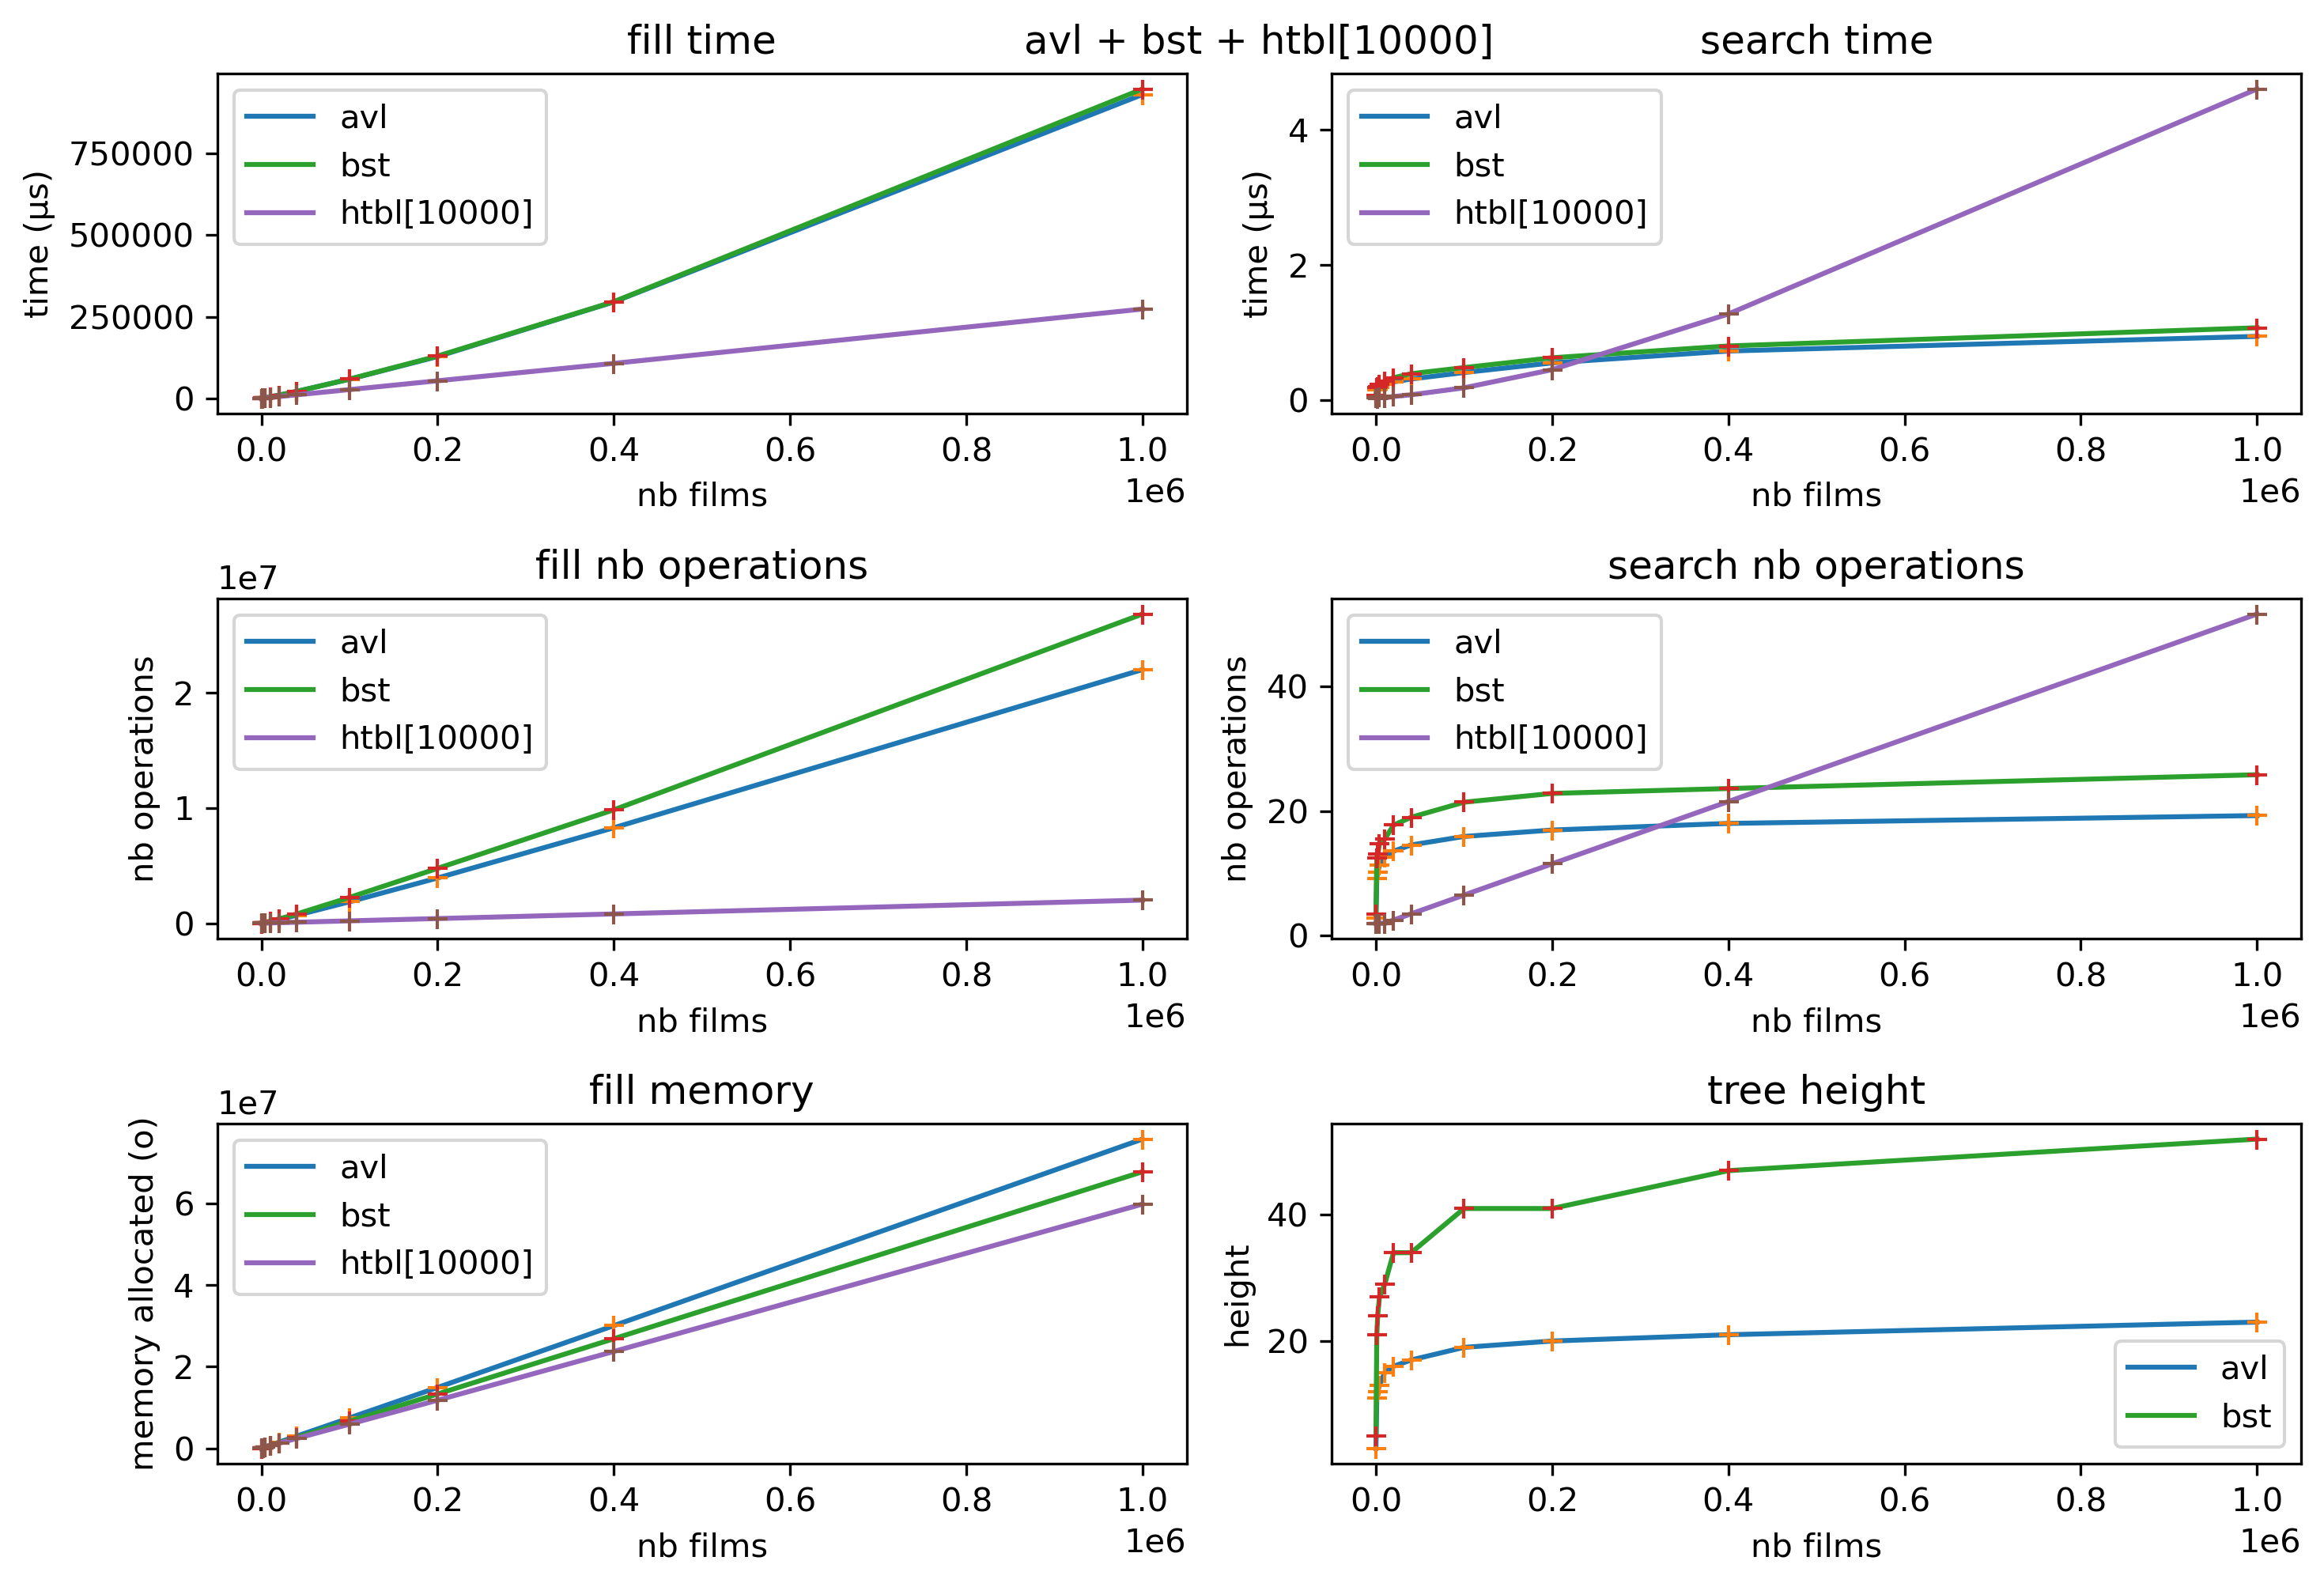
\includegraphics[width=1.0\textwidth]{../plots/nb_search_500_000/bst_avl_htbl.png}
            
                \caption{Résultats des mesures pour les trois structures, avec \texttt{nb\_search=500 000}.}
                \label{fig:avl_bst_htbl}
            \end{figure}

            On remarque que les arbres (AVL et ABR=BST) ont des comportements similaires et se distinguent de la table de hachage (htbl).

            \vspace{12pt}
            
            $\bullet$ \textbf{Insertion} (\emph{fill}) : comme on ne regarde pas l'insertion d'un élément dans une structure de taille $n$, mais l'insertion des $n$ éléments dans la structure, c'est linéaire pour toutes les structures.

            On remarque que c'est plus rapide pour les tables de hachage : en effet, il y a moins d'opérations à faire lors de l'ajout d'un élément.

            Au niveau de la mémoire : c'est presque la même chose pour les trois, comme on stocke les mêmes données.

            \vspace{12pt}
            
            $\bullet$ \textbf{Recherche} (\emph{search}) : la recherche d'un élément dans une table de hachage semble être en $\mathcal O(n)$ (avec $n$ le nombre d'éléments dans la table), ce qui correspond à la théorie. 

            Pour les arbres, cela semble être en $\mathcal O(\log n)$, ce qui correspond plus ou moins à la théorie (voir en détail dans \ref{sub:tree_comp}).
        \end{indt} %}}}2

        \begin{indt}{\subsection{Comparaison des structures arborescentes}} %{{{2
            \label{sub:tree_comp}

            \begin{figure}[H]
                \centering
            
                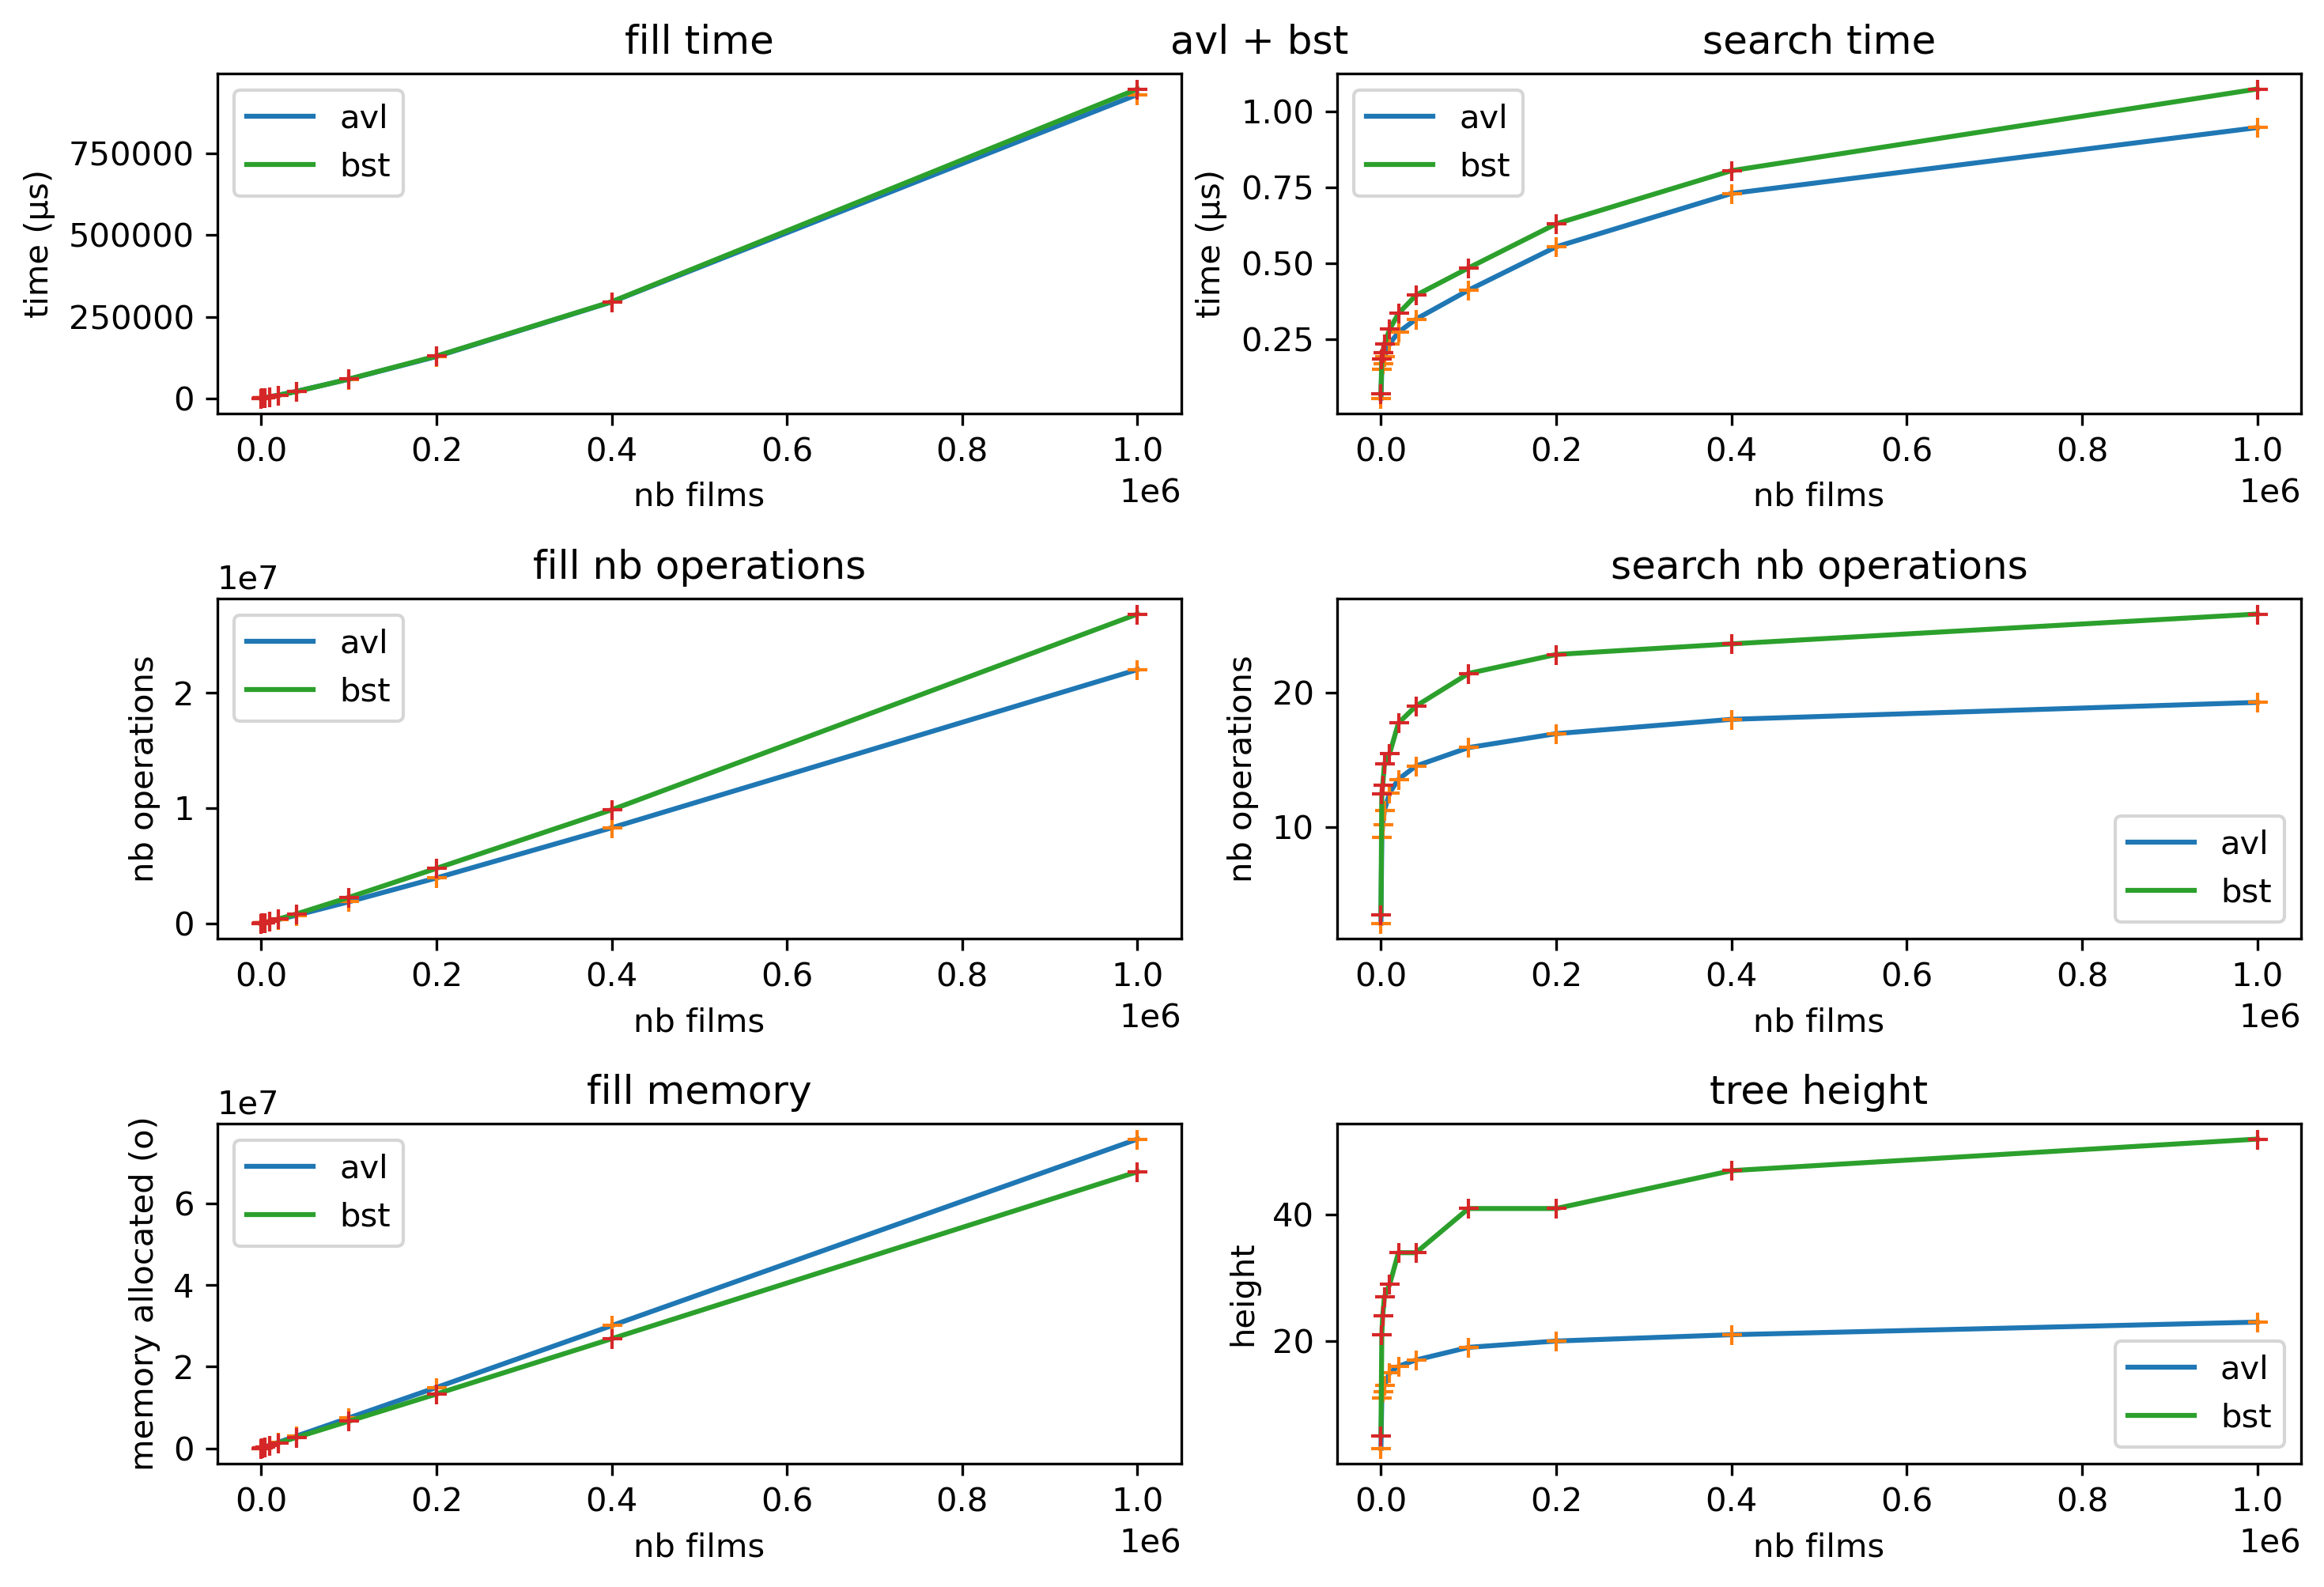
\includegraphics[width=1.0\textwidth]{../plots/nb_search_500_000/bst_avl.png}
            
                \caption{Résultats pour les arbres (AVL et ABR), avec \texttt{nb\_search=500 000}}
                \label{fig:avl_bst}
            \end{figure}

            $\bullet$ \textbf{Insertion} : \textit{cf} \ref{sub:all_comp}.

            $\bullet$ \textbf{Recherche} : la recherche est plus rapide sur les avl, ce qui corrobore donc bien la théorie.

            On remarque aussi que la hauteur des ABR est en $\mathcal O(\log n)$ (avec $n$ le nombre d'éléments dans l'arbre) avec ces données.

            Mais la hauteur des ABR est de l'ordre de deux fois plus que celle des AVL, pour un même nombre de données.
            Cela se traduit bien par une recherche plus rapide pour les AVL.

            \vspace{12pt}
            
            On peut regarder plus en détail, en faisant la différence entre les bst et les avl :
            \begin{figure}[H]
                \centering
            
                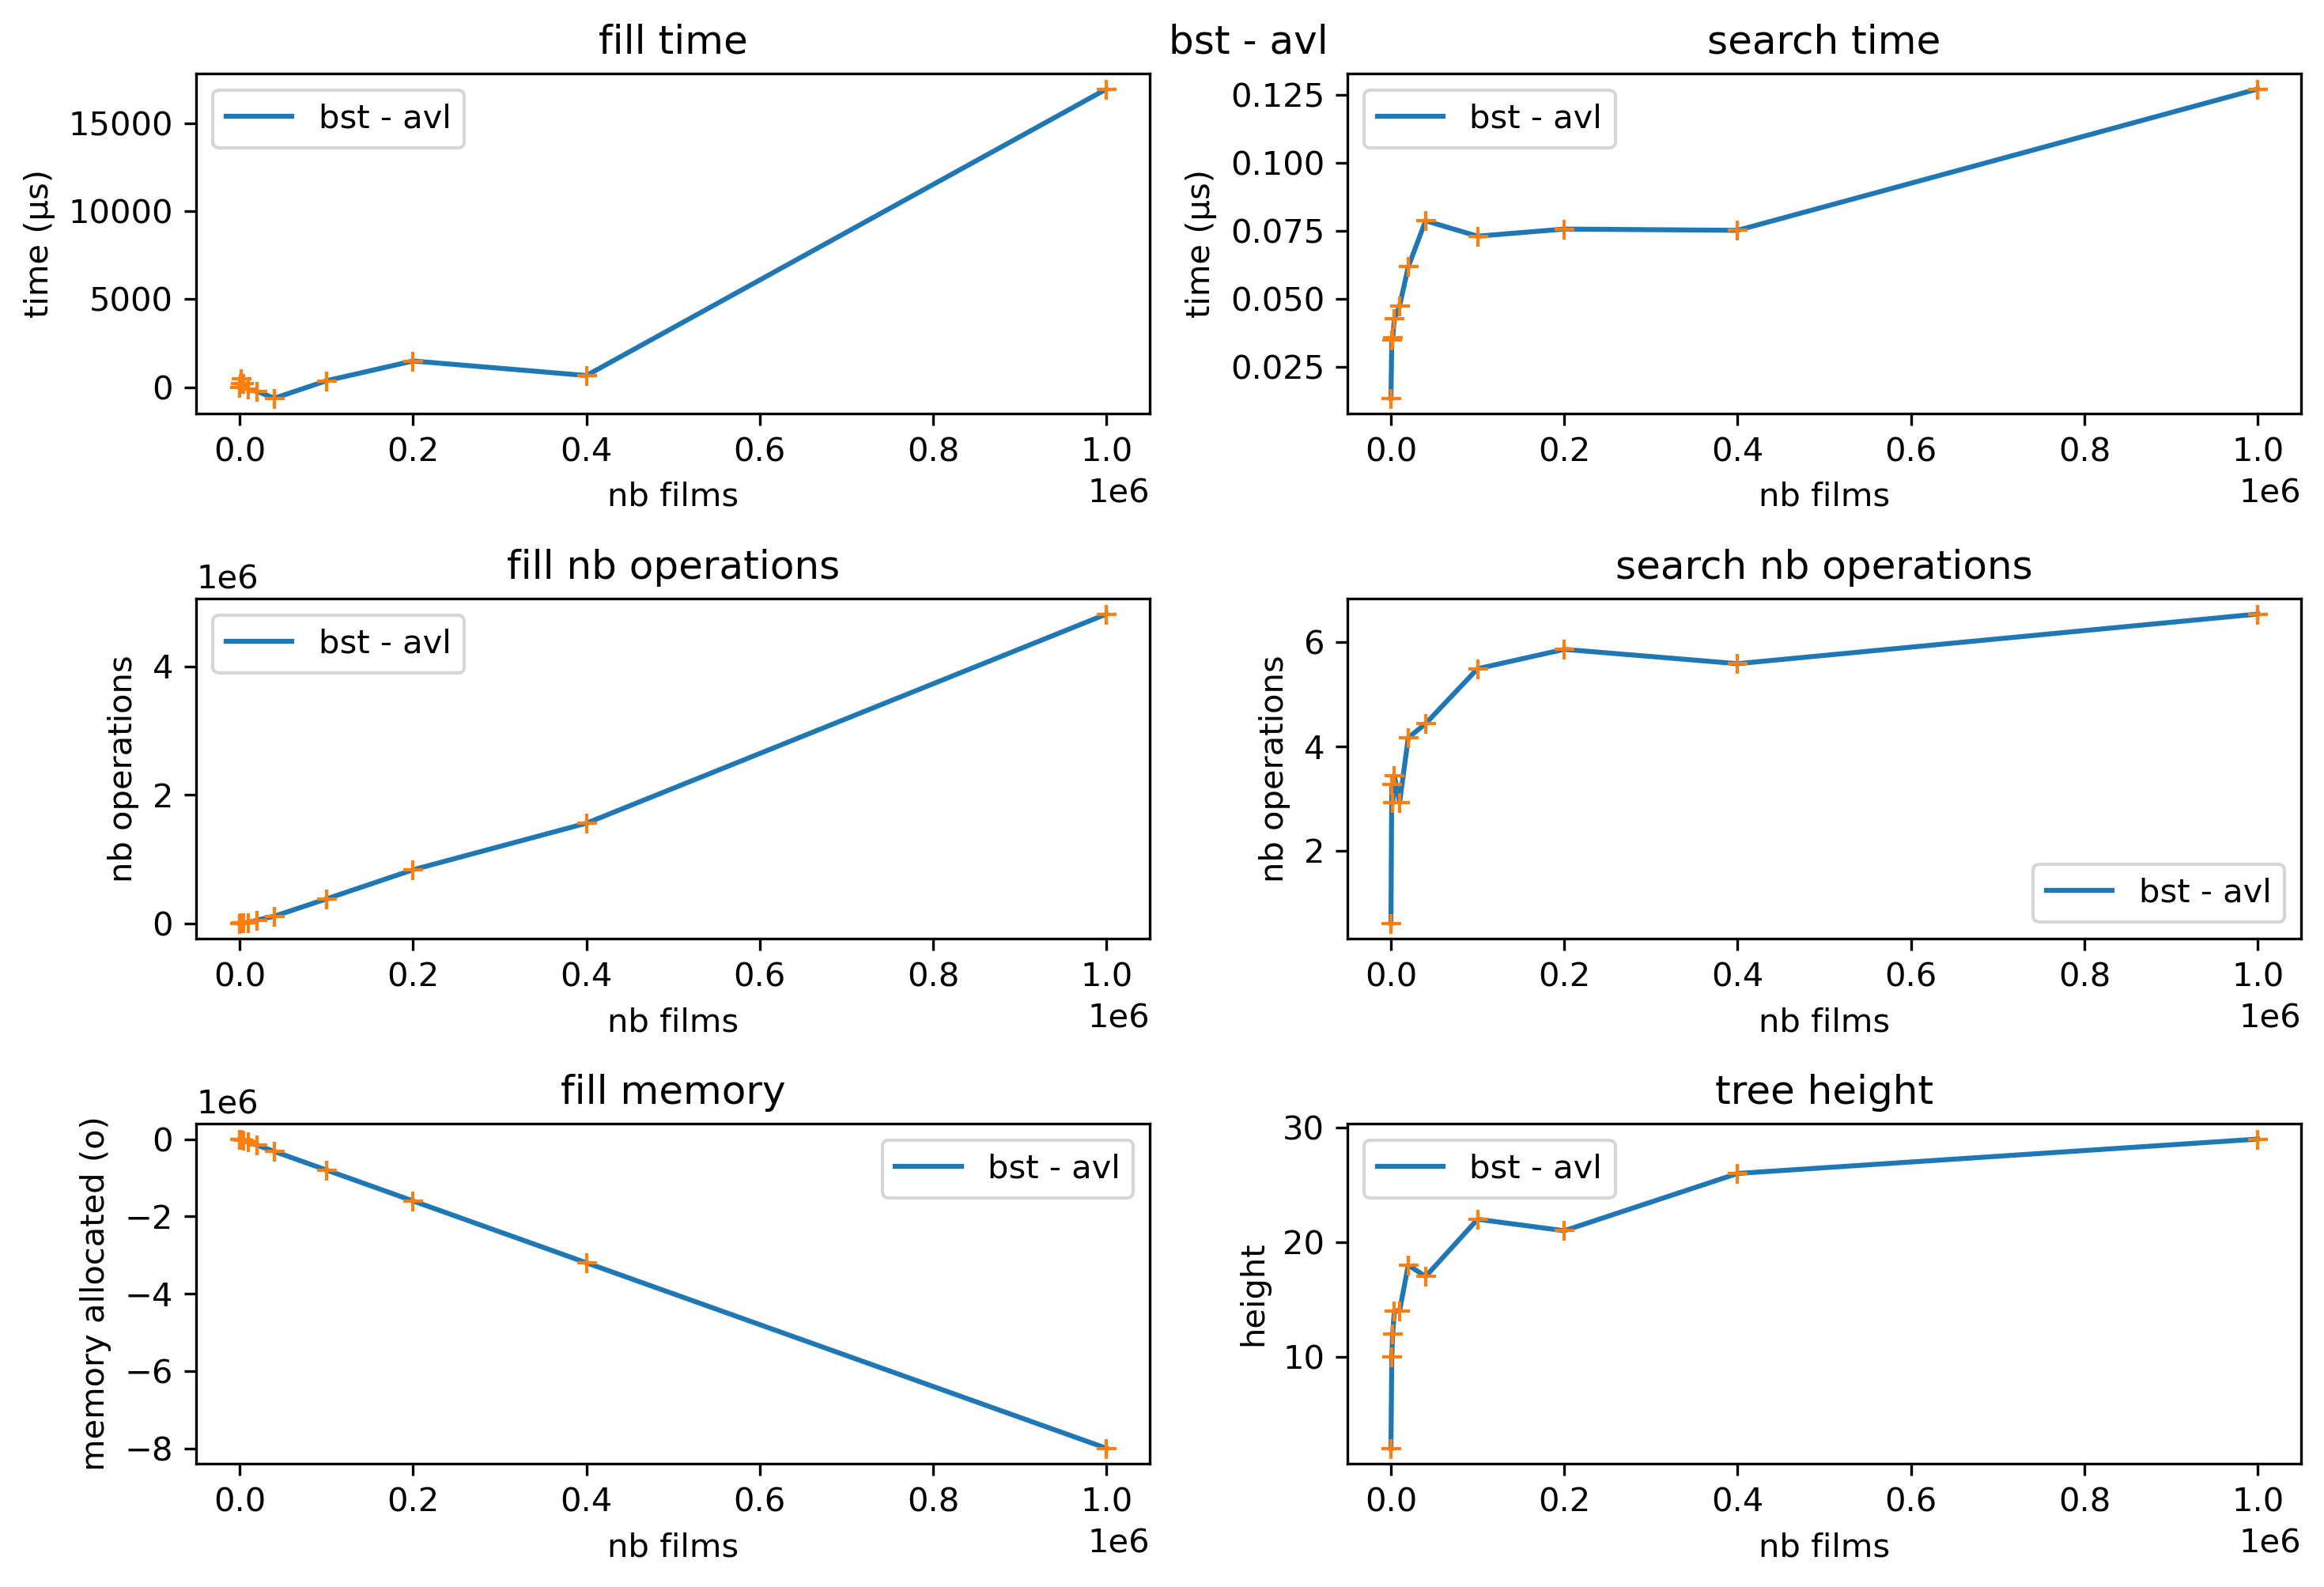
\includegraphics[width=1.0\textwidth]{../plots/nb_search_500_000/bst_minus_avl.png}
            
                \caption{Différence entre ABR et AVL (\texttt{nb\_search=500 000})}
                \label{fig:bst_minus_avl}
            \end{figure}

            On remarque que la différence entre les hauteurs est même en $\mathcal O(\log n)$.
        \end{indt} %}}}2

        \begin{indt}{\subsection{Comparaison des tables de hachage}} %{{{2
            \begin{figure}[H]
                \centering
            
                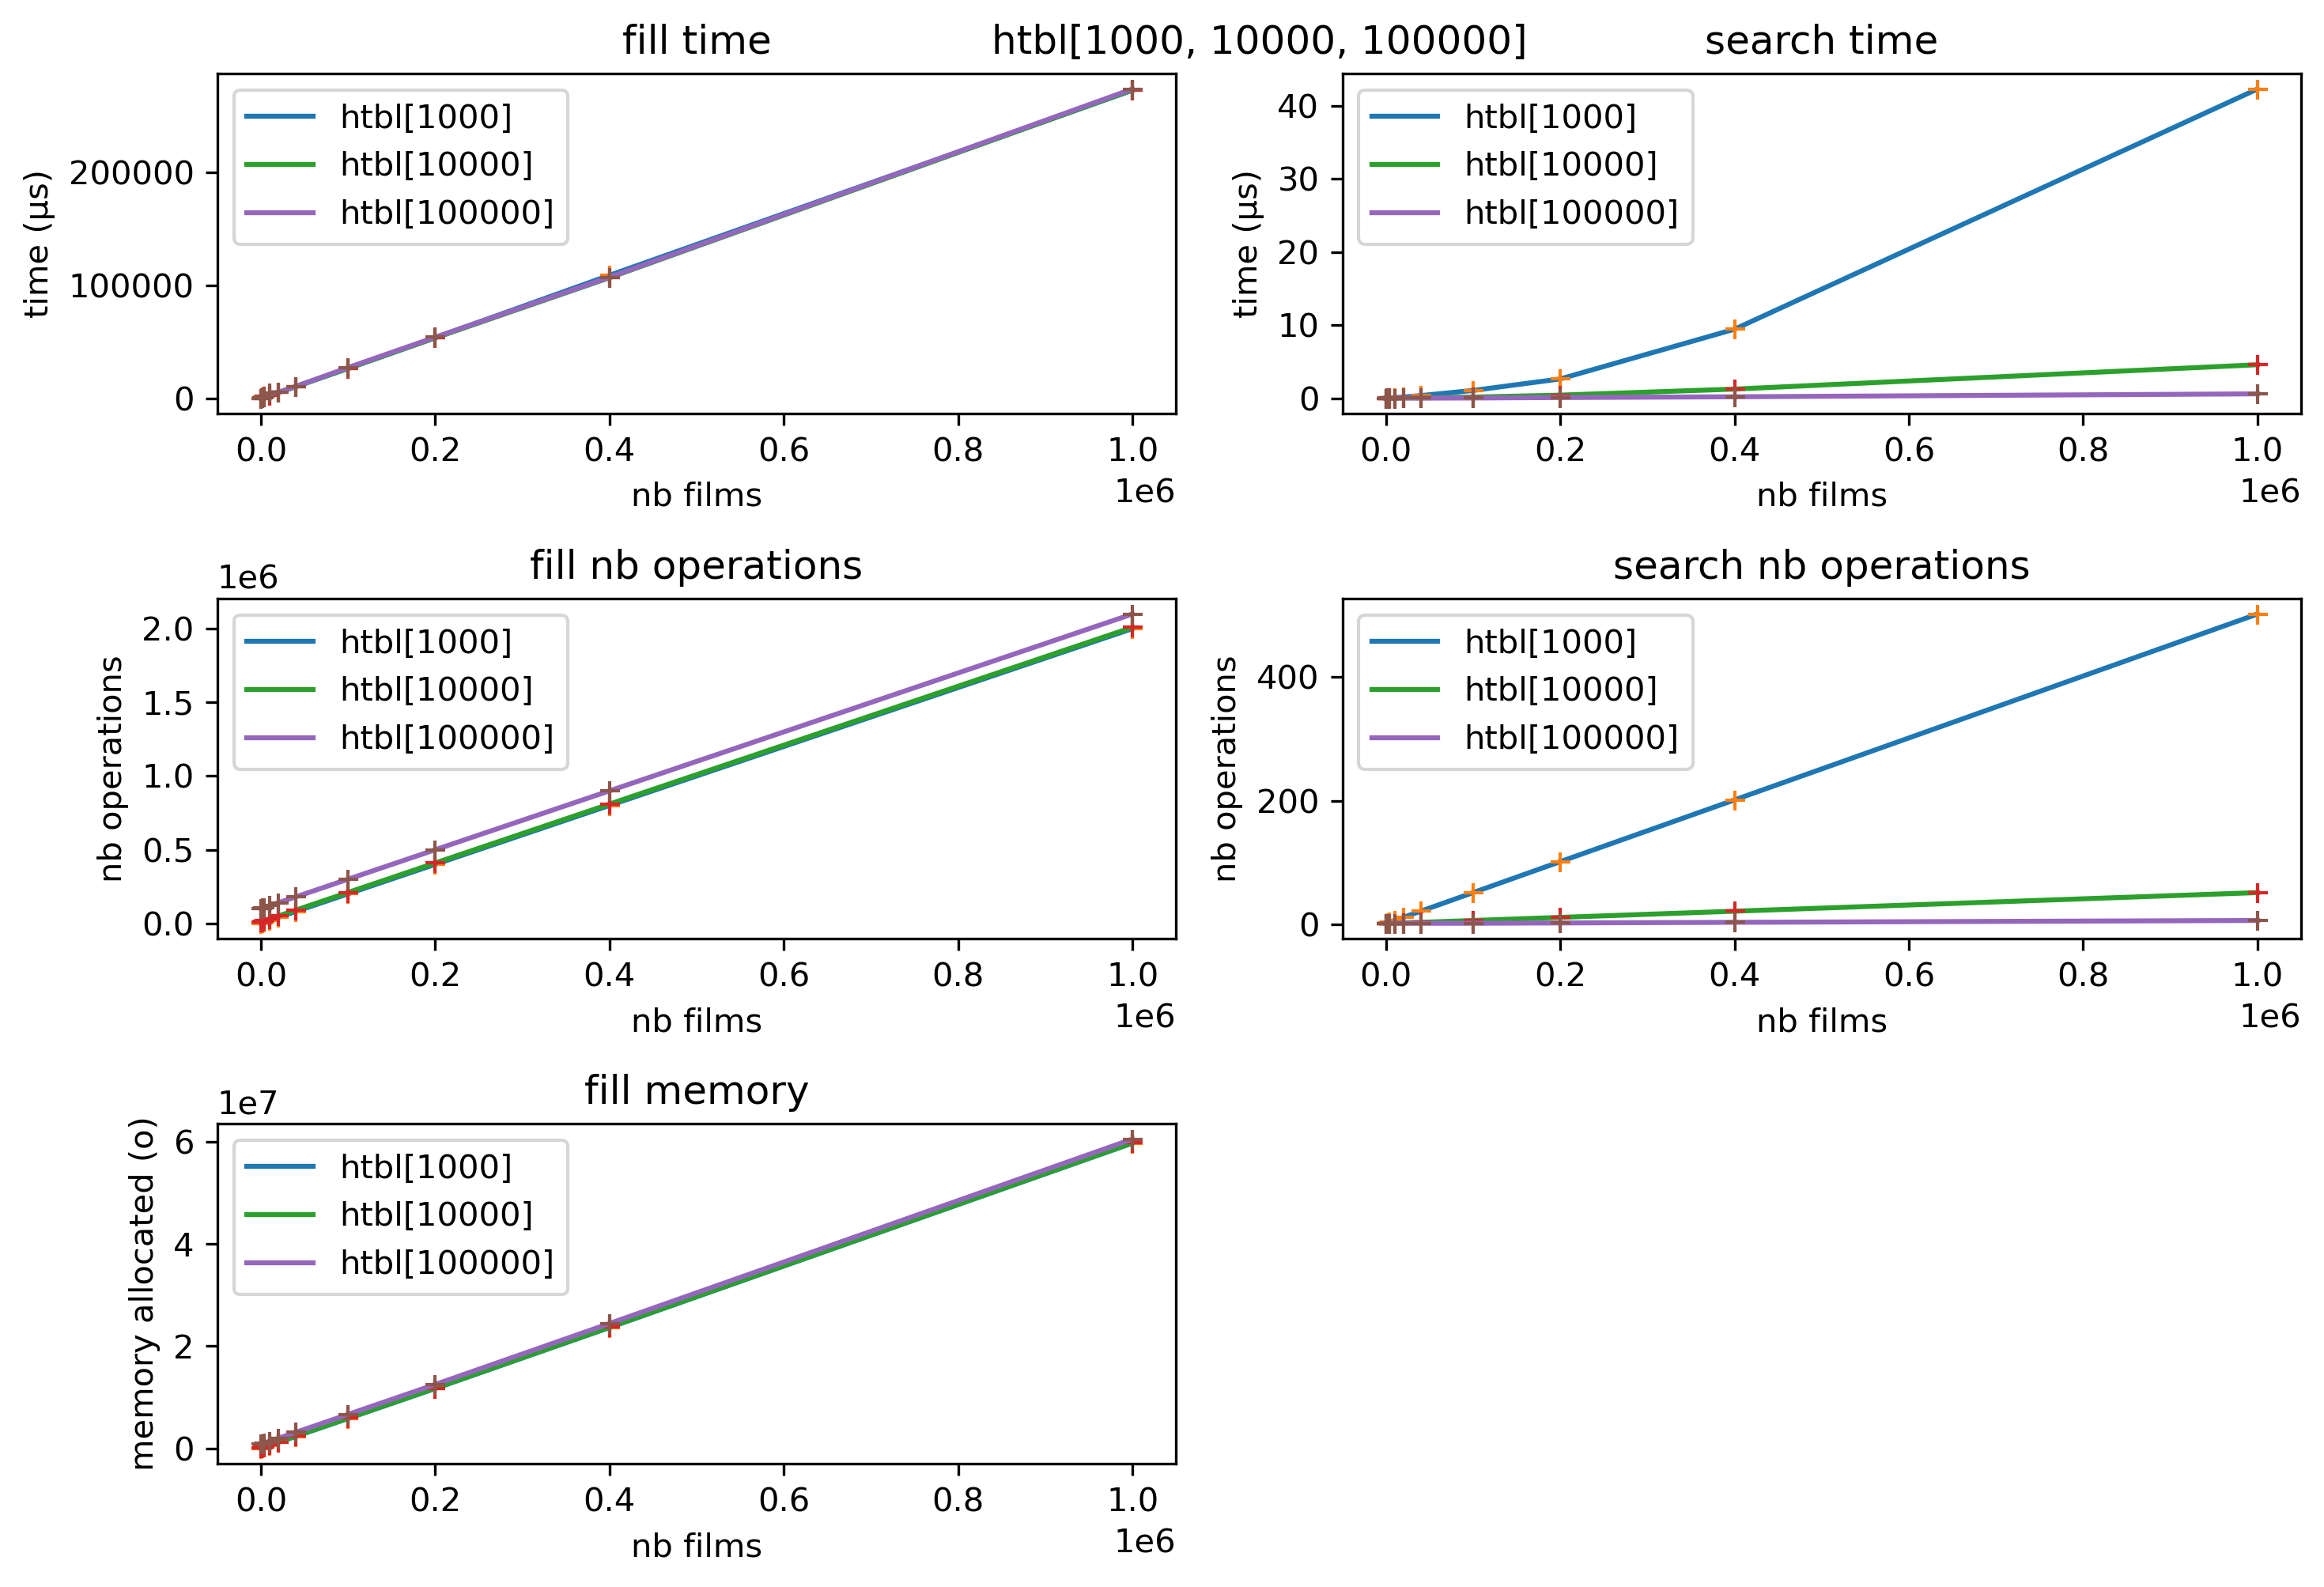
\includegraphics[width=1.0\textwidth]{../plots/nb_search_500_000/htbl.png}
            
                \caption{Résultats pour les tables de hachage avec différentes tailles (\texttt{nb\_search=500 000})}
                \label{fig:htbl}
            \end{figure}

            Tout est linéaire en le nombre de données dans la structure, mais il semblerait qu'une taille plus grande donne de meilleurs résultats.
            En effet, on aura moins de collisions, mais la table prendra plus de place.

            On peut tracer les courbes en fonction de la taille de la table au lieu du nombre de données :

            \begin{figure}[H]
                \centering
            
                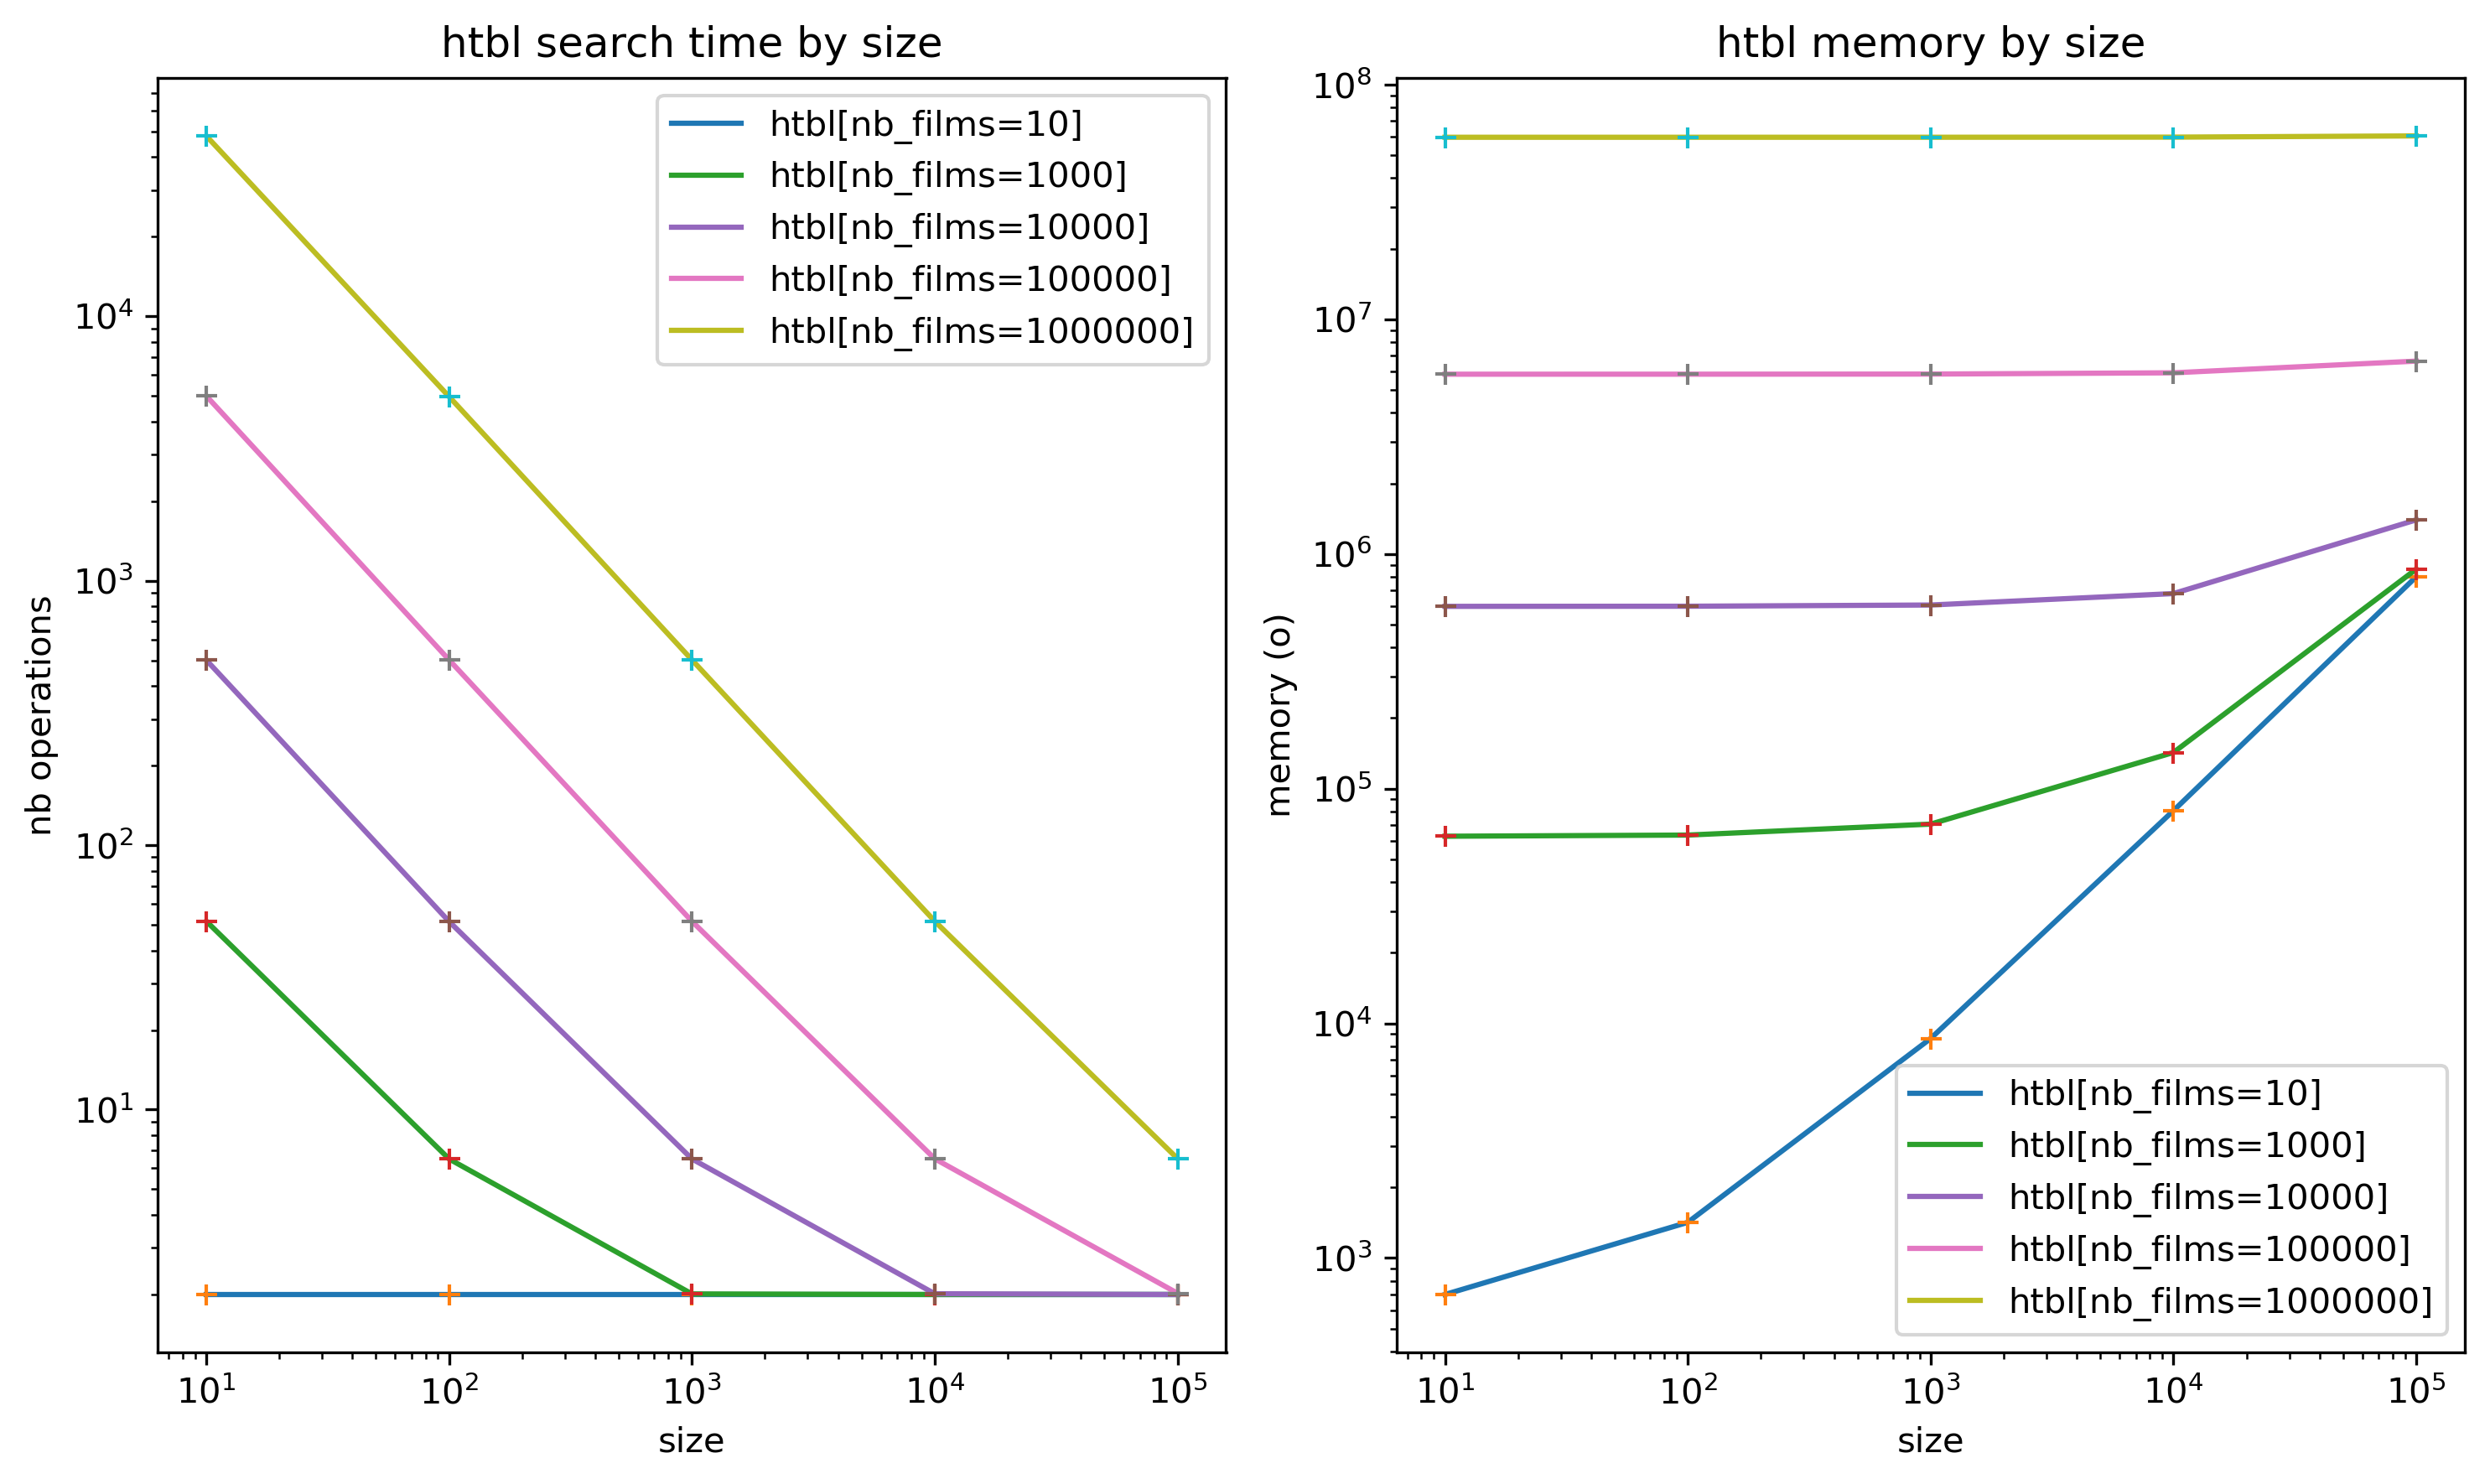
\includegraphics[width=1.0\textwidth]{../plots/nb_search_500_000/htbl_size.png}
            
                \caption{Nombre d'opérations et mémoire des tables de hachage en fonction de la taille (échelle logarithmique)}
                \label{fig:htbl_size}
            \end{figure}

            Si on a peu de données (courbe \texttt{htbl[nb\_films=10]} par exemple), alors augmenter la taille ne rend pas pas la recherche plus rapide, mais prend de la place pour rien.

            Si on a beaucoup de données, (courbe \texttt{htbl[nb\_films=100000]} par exemple), alors augmenter la taille de la table de hachage permet de réduire les collisions et ainsi d'augmenter la vitesse de recherche.
            On remarque que dans ce cas, la taille n'influe pas sur la mémoire allouée (car il n'y a jamais de collisions).
        \end{indt} %}}}2
    \end{indt} %}}}1
    
\end{document}
%--------------------------------------------End

% vim:foldmethod=marker:foldlevel=0
